\clearpage

\section{\label{dataset}Datasets and Event Selection}

The dataset used in this analysis is P16id production of 2014 Au+Au 200 GeV data. This is the first year of physics running the new STAR HFT Detector. The analysis uses picoDst which is produced from MuDst.

The Minimum-Bias (MinBias) trigger is defined as a coincidence between the two VPDs, and an online collision vertex cut. Moreover, a pile-up protection at the trigger level was applied for the data taking. In this analysis, the MinBias trigger, denoted as ``vpdmb-5-p-nobsmd" and ``vpdmb-5-p-nobsmd-hlt", is used. The triggers used in this analysis are listed in Table~\ref{trigger}.

\begin{table}[htp]
\centering
\caption{Triggers ID used in this analysis from run14}
\label{trigger}
	\begin{center}
	\begin{tabular}{l|l}
%  \Xhline{1.6pt}
	Trigger ID	& description\\ \hline
	450050		& vpdmb-5-p-nobsmd-hlt\\ \hline
	450060		& vpdmb-5-p-nobsmd-hlt\\ \hline
	450005		& vpdmb-5-p-nobsmd\\ \hline
	450015		& vpdmb-5-p-nobsmd\\ \hline
	450025		& vpdmb-5-p-nobsmd\\ \hline
%  \Xhline{1.6pt}
	\end{tabular}
	\end{center}
\end{table}

Events used in this analysis are required to have a valid collision vertex $V_{z}$ (primary vertex) within 6 cm of the TPC center along $z$ direction (the beam direction) to ensure a uniform TPC acceptance and make sure the most tracks are within the PiXeL (PXL) detector coverage. The PXL detector is about 20 cm along the z direction, and the radius of the inner layer is about 2.8cm and outer layer is about 8 cm. Furthermore, the distance between the $V_{z}$ constructed by TPC and the vertex constructed by VPD ($V_{z}^{VPD}$, fast detector) is within 3 cm to reject the bad events. A radial length less than 2 cm for the vertex is required to reject the events from the beam hitting the beam pipe. After event selection, $\sim$875 million MinBias events are used for this analysis. Table~\ref{eventselection} lists the event selection criterion.

\begin{table}[htp]
\centering
\caption{Event selection in Au+Au collisions at 200 GeV for $D^0$.}
\label{eventselection}
\begin{tabular}{c}
\toprule[1.6pt]
Event Selection Criteria \\
\midrule[1.2pt]
\multirow{2}*{$!(|V_{x}|== 0 \ \&\& \ |V_{y}|== 0 \  \&\& \  |V_{z}|== 0) $ } \\
\\
\multirow{2}*{$|V_{z}|<$ 6 cm} \\
\\
\multirow{2}*{$|V_{r}|<$ 2 cm} \\
\\
\multirow{2}*{$|V_{z} - V_{z}^{VPD}|<$ 3 cm} \\ 
\\  
\bottomrule[1.6pt]
\end{tabular}
\end{table}

\subsection{Centrality Definition}

The centrality for Run14 200GeV Au+Au collisions MinBias sample is based on gRefMult. The gRefMult is defined as the number of global tracks with $|\eta|<0.5$, no less than 10 TPC hits, and Distance of Closest Approach (DCA) to primary vertex less than 3 cm with some correction according to $V_{z}$ and luminosity. The centrality definition according to the corrected gRefMult is listed in Table ~\ref{centrality}. This is decided by comparing the measured gRefMult distribution with the Glauber model simulation. 

The basic procedure for centrality definition have three steps. First, need the quality assurance (QA) for the data set and remove those outlier runs. The second step would be correct the $V_{z}$ and luminosity dependence for the reference multiplicity (gRefmult). The last step would be compare our data with Glauber MC simulation and determine the centrality classification.

For the QA, several variables are used for the outlier selection, such as Refmult (primary track multiplicity), gRefmult (global track multiplicity), TofRefmult (tof track multiplicity) and etc. In the Fig.~\ref{fig:centrality_QA1} shows the $\langle$gRefmult$\rangle$ as a function of run index for the QA, and there are several outliers are identified. Those dashed lines are the 4$\times$RMS range, beyond those range, the runs are identified as bad run. And several iterations are did until all the runs are within these 4$\times$RMS range.


In the Fig.~\ref{fig:centrality_QA2} shows the $\langle$HFT $p_{T}$$\rangle$, which is the mean $p_{T}$ of HFT tracks, as a function of run index for the QA, and we can clearly see there is a deep before the run index $\sim$520 which corresponding to the run number 15107008. And also we saw the same structure in the Fig.~\ref{fig:centrality_QA3}, which shows the average of HFT matching Ratio in the $p_{T}$ range between 0.7 to 0.8 GeV/$c$ and Fig.~\ref{fig:centrality_QA4} shows this HFT matching ratio in the high $p_{T}$ range. So, basically those runs before day 107 were taken out for this analysis, since it will complicate our efficiency calculation.

This deep was identified later on with a lot of effort, it was due to the firmware issue. And more details can be found in the STAR documents below.

\url{https://drupal.star.bnl.gov/STAR/system/files/STAR_PXL_Firmware_Issue_Solved_Final_Report_Oct3_v2.pdf}

\begin{figure}[htbp]
\begin{minipage}[htbp]{0.52\linewidth}
\centering
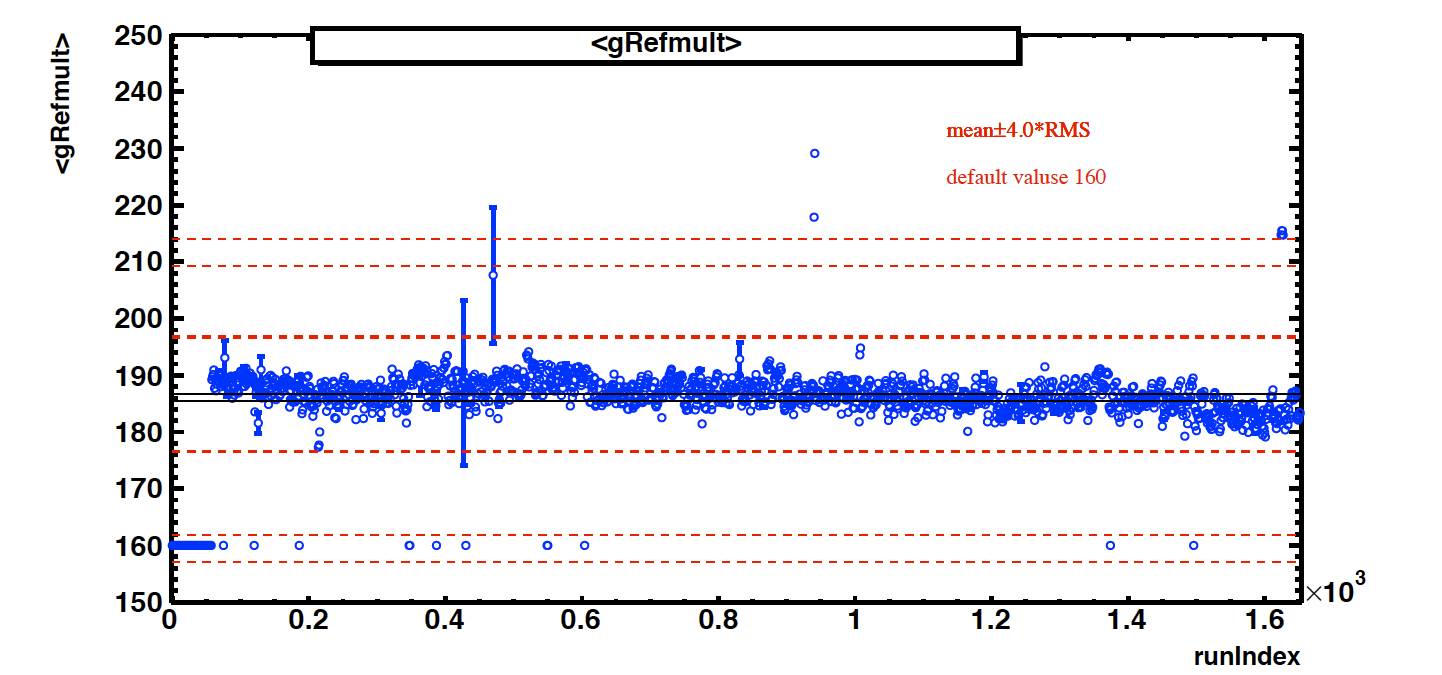
\includegraphics[width=1.0\textwidth]{figure/Run14_D0HFT/centrality_grefmult.png}
\caption{The mean value of gRefmult ($\langle$gRefmult$\rangle$) as a function of run index from QA.\label{fig:centrality_QA1}}
\end{minipage}
\hfill
\begin{minipage}[htbp]{0.52\linewidth}
\centering
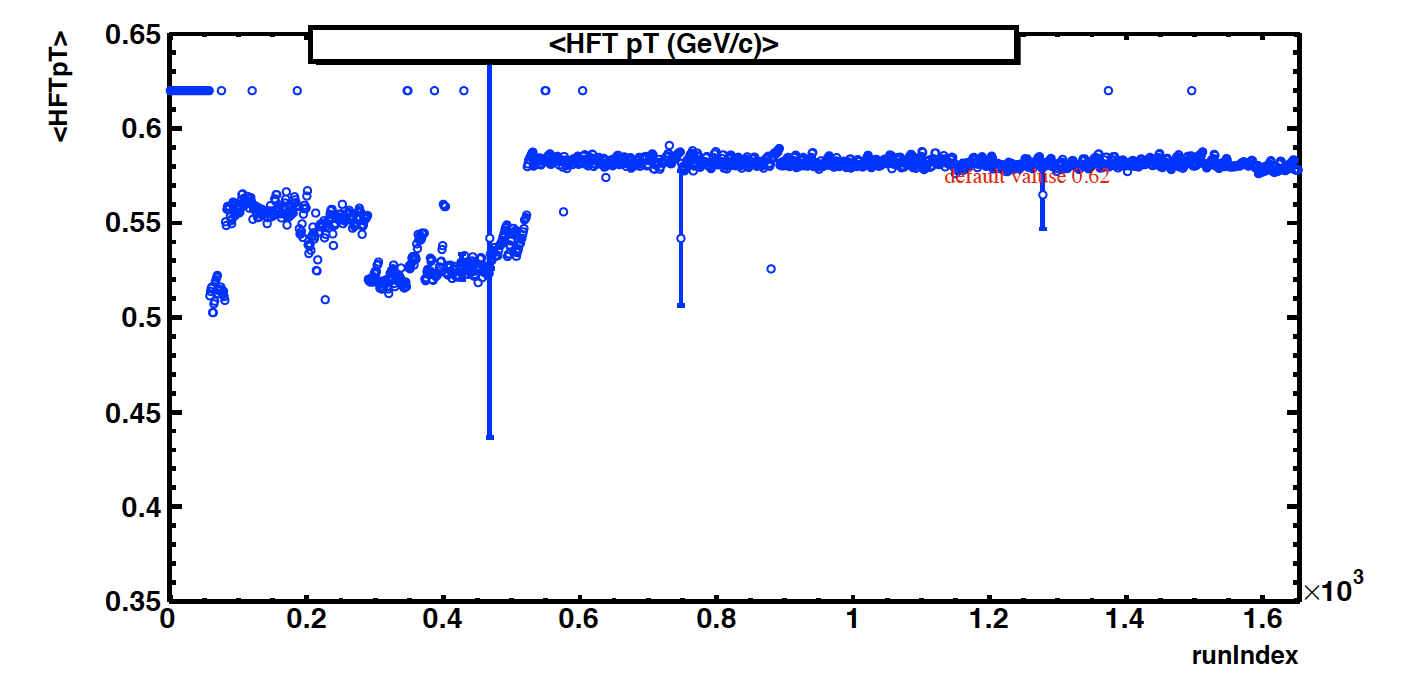
\includegraphics[width=1.0\textwidth]{figure/Run14_D0HFT/centrality_HFTpt.png} 
\caption{The mean value of $p_{T}$ for HFT matched track ($\langle$HFT $p_{T}$$\rangle$) as a function of index.\label{fig:centrality_QA2}}
\end{minipage}
\end{figure}


\begin{figure}[htbp]
\begin{minipage}[htbp]{0.52\linewidth}
\centering
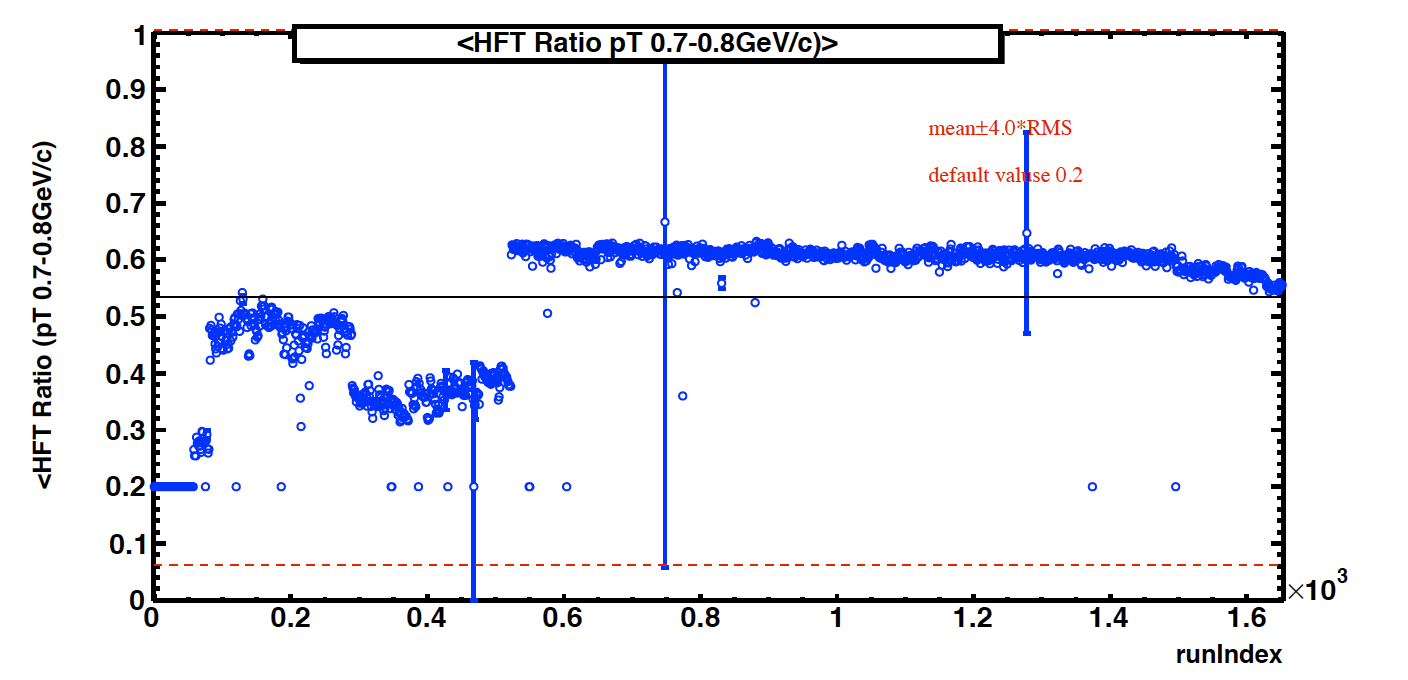
\includegraphics[width=1.0\textwidth]{figure/Run14_D0HFT/centrality_HFTratio.png}
\caption{The HFT matching ratio at the transverse momentum range 0.7 < $p_{T}$ < 0.8 GeV/$c$ as a function of run index .\label{fig:centrality_QA3}}
\end{minipage}
\hfill
\begin{minipage}[htbp]{0.52\linewidth}
\centering
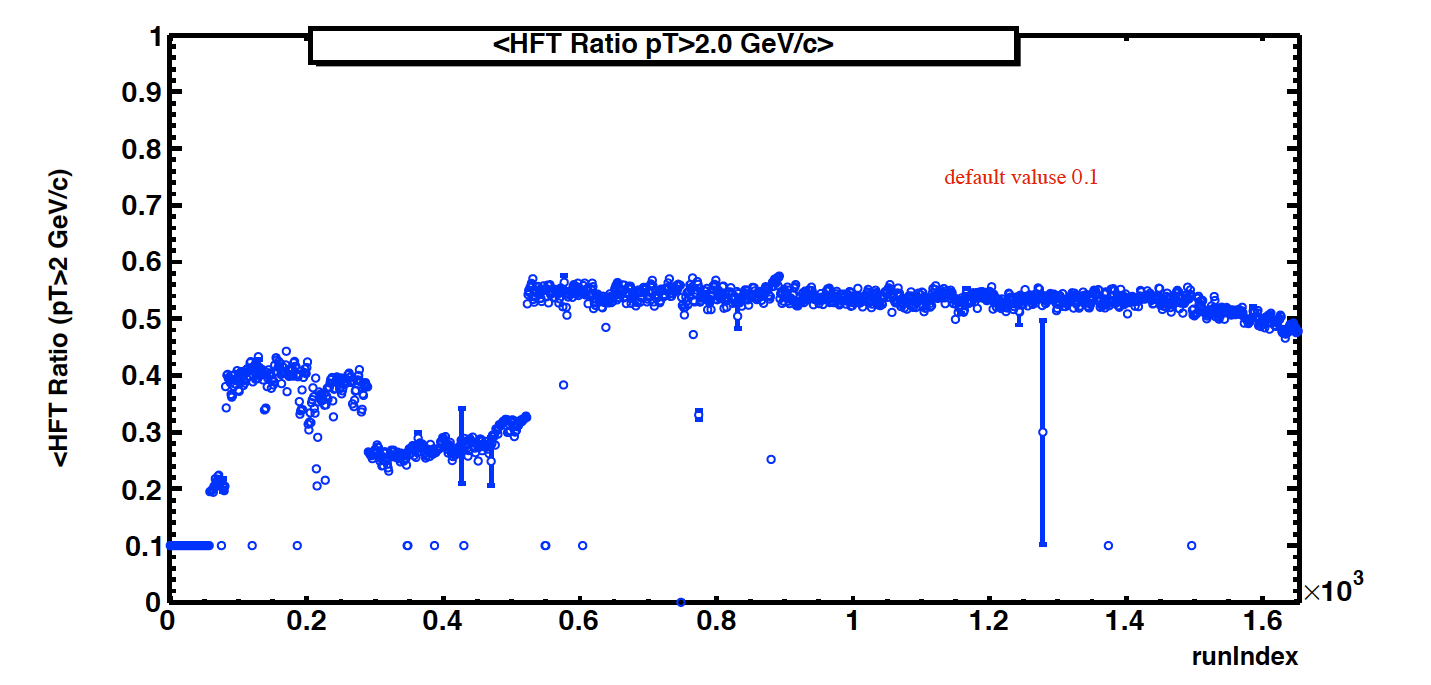
\includegraphics[width=1.0\textwidth]{figure/Run14_D0HFT/centrality_HFTratio2.png} 
\caption{The mean value of HFT matching ratio at the transverse momenaum range $p_{T}$ $\sim$2.0 GeV/$c$ as a function of run index .\label{fig:centrality_QA4}}
\end{minipage}
\end{figure}

Fig.~\ref{fig:MB5_vz} and Fig.~\ref{fig:MB30_vz} show the normalized gRefmult distribution for several different $V_{z}$ range from -6 cm to 6 cm. The shape are quite different for VpdMB5 trigger in Fig.~\ref{fig:MB5_vz} while the Fig.~\ref{fig:MB30_vz} shows the same plots for VpdMB30 trigger ($V_z$ within range from -30 cm to 30 cm). This difference was explained by that the online Vpd vertex cut have a negative offset and the Vpd resolution has centrality dependence. As for the most central collisions, the resolution will be better than the most peripheral collisions. That is the reason we saw more events in the negative $V_{z}$ range and more central events for VpdMB5 trigger compared to VpdMB30 trigger.

\begin{figure}[htbp]
\begin{minipage}[htbp]{0.52\linewidth}
\centering
% 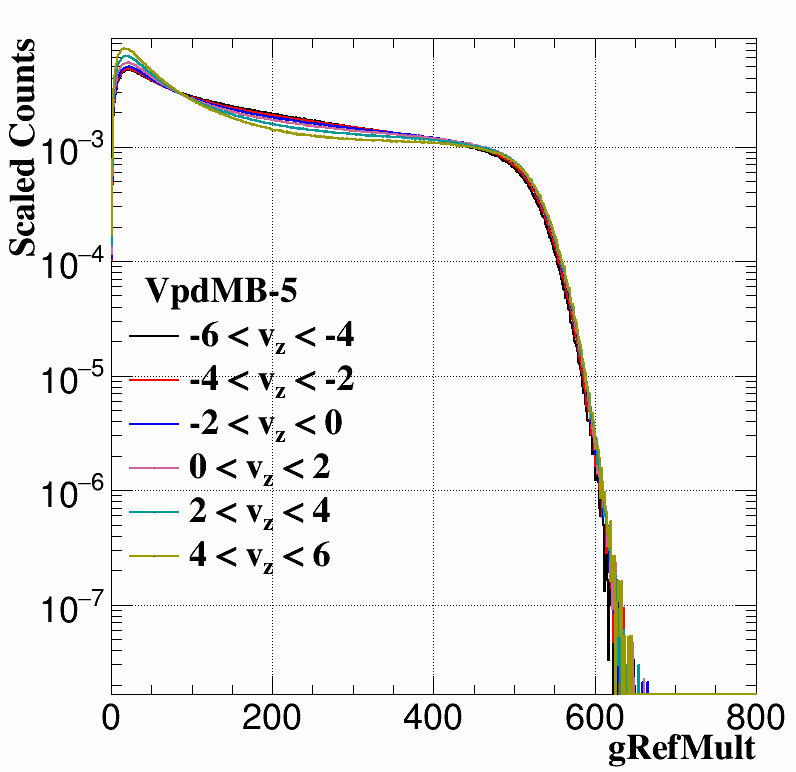
\includegraphics[width=0.75\textwidth]{figure/Run14_D0HFT/MB5_gref.png}
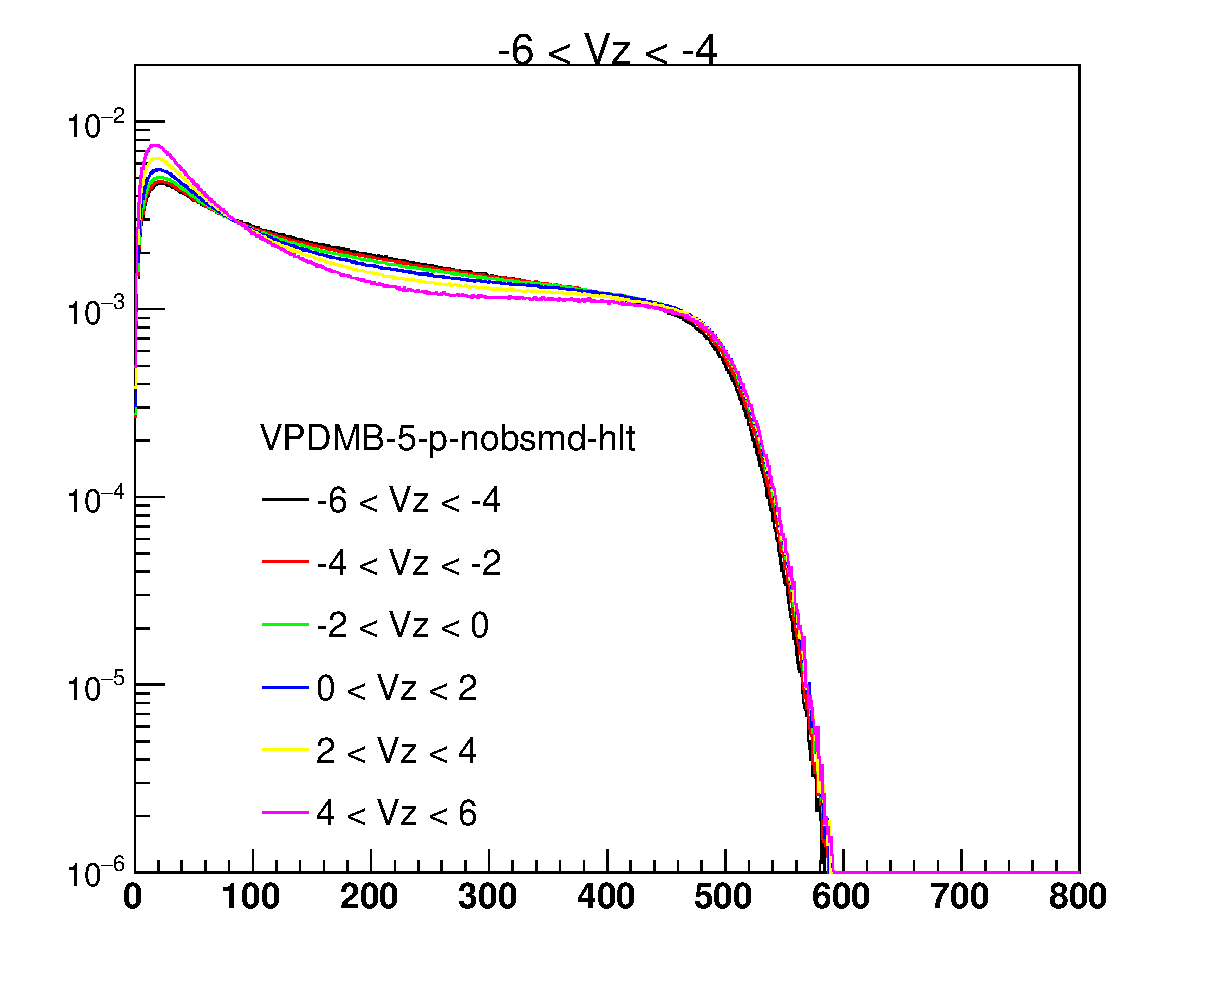
\includegraphics[width=0.75\textwidth]{figure/Run14_D0HFT/gREfMult_Diffferent_Vz_VPDMB-5-p-nobsmd-hlt.eps}
\caption{Normalized gRefmult distribution for VpdMB5 trigger along different $V_{z}$ range\label{fig:MB5_vz}}
\end{minipage}
\hfill
\begin{minipage}[htbp]{0.52\linewidth}
\centering
% 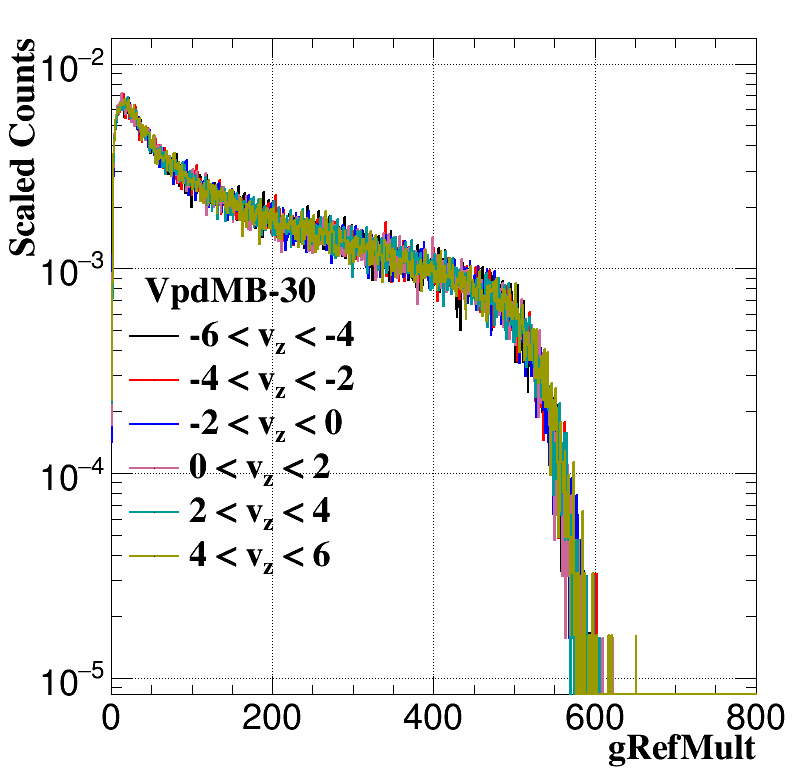
\includegraphics[width=0.75\textwidth]{figure/Run14_D0HFT/MB30_gref.png} 
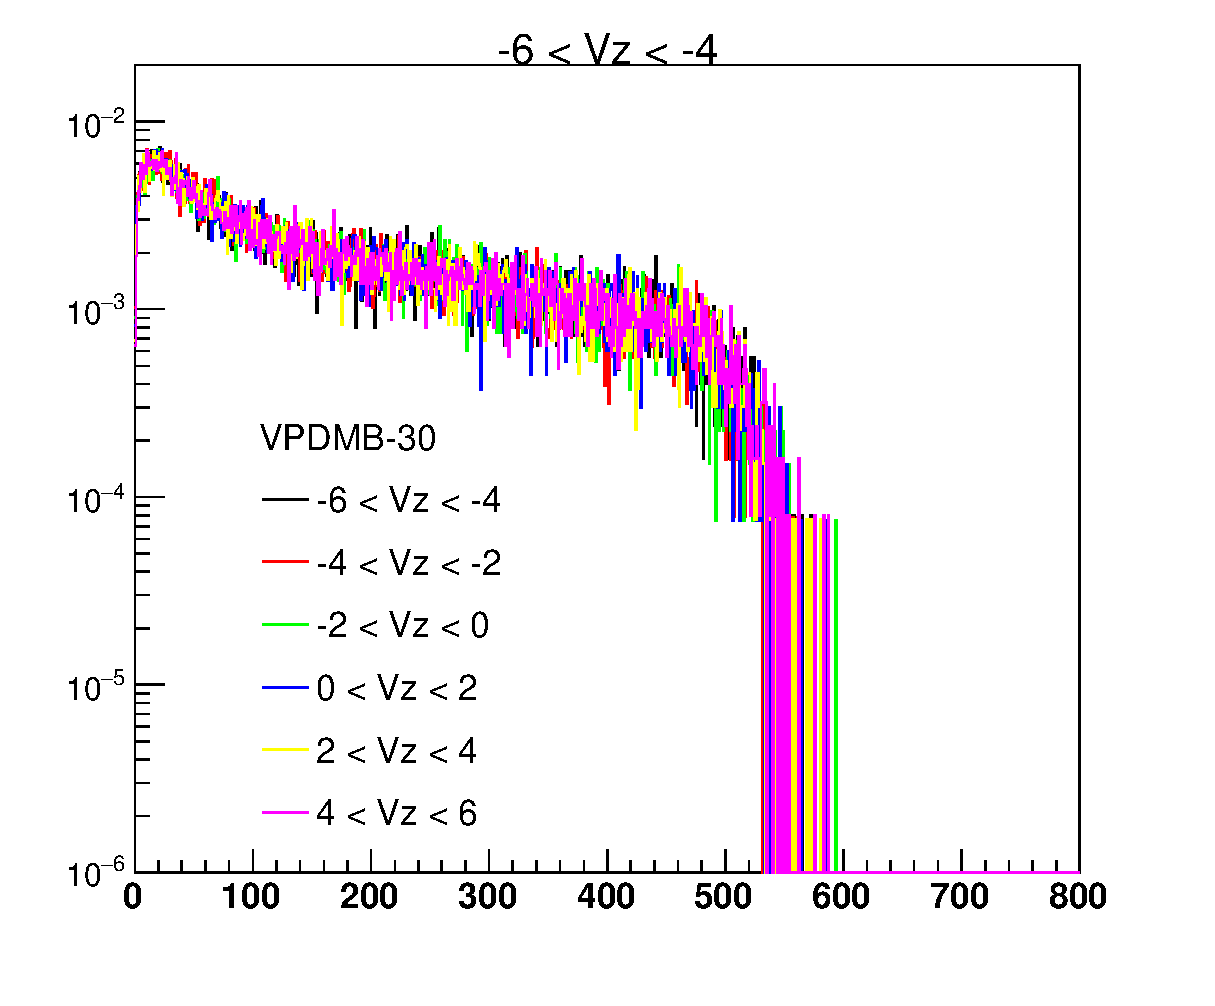
\includegraphics[width=0.75\textwidth]{figure/Run14_D0HFT/gREfMult_Diffferent_Vz_VPDMB-30.eps} 
\caption{Normalized gRefmult distribution for VpdMB30 trigger along different $V_{z}$ range\label{fig:MB30_vz}}
\end{minipage}
\end{figure}

As the gRefmult have the luminosity dependence (related to the TPC tracking efficiency have luminosity dependence), we need to take out this effect by doing ZdcX (Zdc coincidence rate) correction. Fig.~\ref{fig:MB5_zdc1} shows the mean value of gRefmult (<gRefmult>) distribution as a function of ZdcX. There was a clear slope for this distribution as shown by the fitting parameters. Here the fitting function is Eq.~\ref{funzdc},
\begin{equation}
f_{ZdcX} = p0 + p1*ZdcX
\label{funzdc}
\end{equation}
The goal of this correction is try to flatten this ZdcX dependence to take out of the luminosity effect. So here the correction factor was shown by  Eq.~\ref{funzdc2}.
\begin{equation}
f_{ZdcX} = \frac{1}{1 + p1/p0*ZdcX}
\label{funzdc2}
\end{equation}
After the ZdcX correction, this <gRefmult> is flat as shown by Fig.~\ref{fig:MB5_zdc2}.

For the $V_{z}$ dependence correction, we extract the high end point (h) from the fitting of gRefmult tail by the function of Eq.~\ref{funerf}.
\begin{equation}
f_{x} = A * TMath::Erf(-\sigma*(x-h)) + A
\label{funerf}
\end{equation}

\begin{figure}[htbp]
\begin{minipage}[htbp]{0.52\linewidth}
\centering
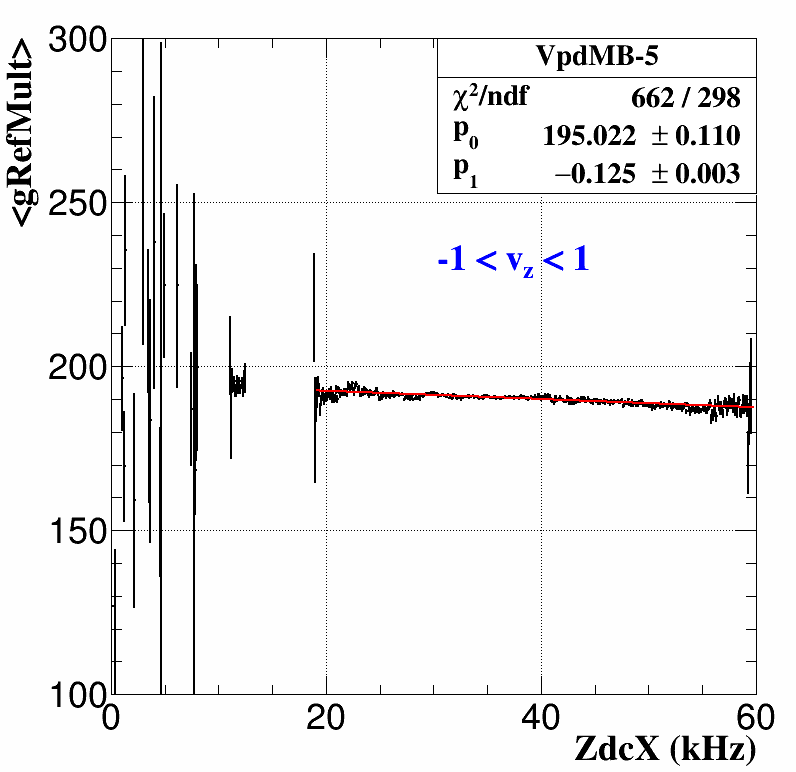
\includegraphics[width=0.75\textwidth]{figure/Run14_D0HFT/MB5_ZDCcor1.png}
\caption{<gRefmult> as function of ZdcX before correction.\label{fig:MB5_zdc1}}
\end{minipage}
\hfill
\begin{minipage}[htbp]{0.52\linewidth}
\centering
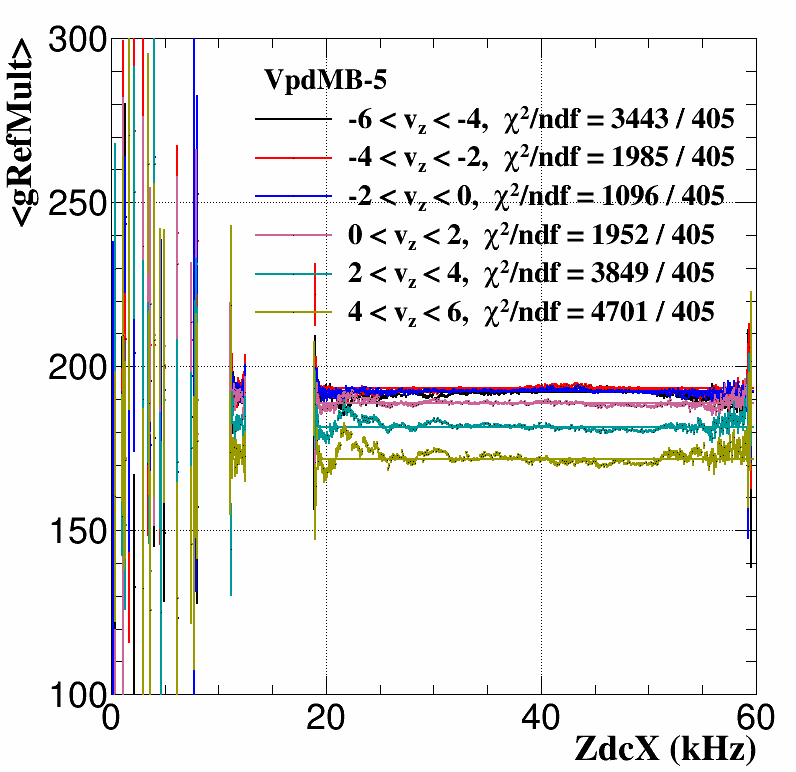
\includegraphics[width=0.75\textwidth]{figure/Run14_D0HFT/MB5_ZDCcor2.png} 
\caption{<gRefmult> as function of ZdcX after correction.\label{fig:MB5_zdc2}}
\end{minipage}
\end{figure}

Fig.~\ref{fig:MB5_vz1} shows an example of the fitting of gRefmult tail in the $V_{z}$ range from 1 cm to 2 cm. The fitting parameters were shown on the plot.

\begin{figure}[htbp]
\centering
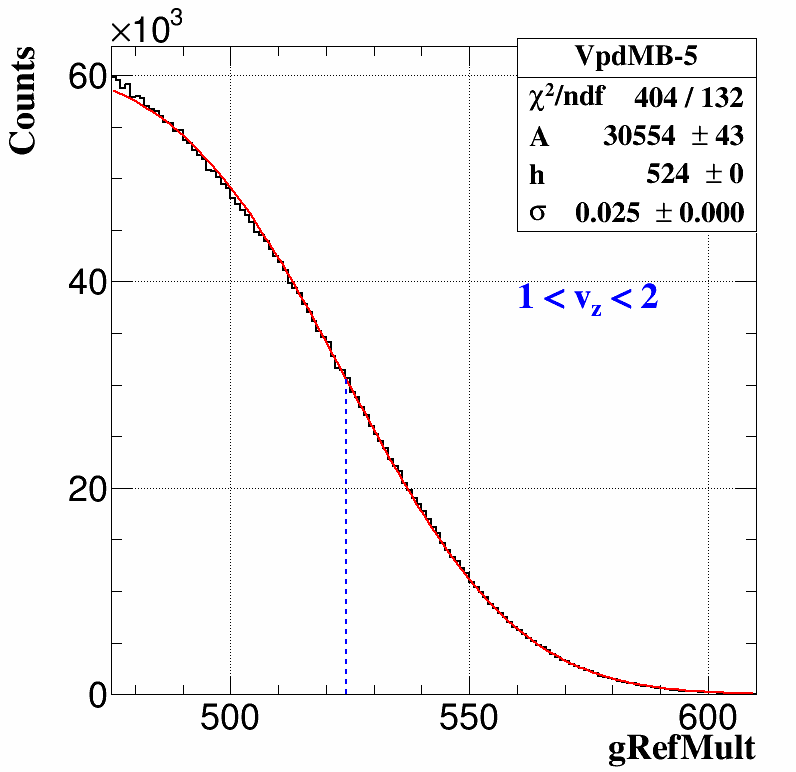
\includegraphics[keepaspectratio,width=0.5\textwidth]{figure/Run14_D0HFT/MB5_Vzcor1.png}
\caption{Fitting gRefmult tail distribution in the range of 1<$V_{z}$<2 cm by Eq.~\ref{funerf}.}
 \label{fig:MB5_vz1}
\end{figure}

With all the high end point value extracted along $V_{z}$ direction, this $V_{z}$ dependence was shown on Fig.~\ref{fig:MB5_vz2}. The similar method as ZdcX correction, we need to flatten this $V_{z}$ dependence, then the data point was fitted by 5th order polynomial function Eq.~\ref{funvz}, and then the correction factor was shown by Eq.~\ref{funvz2}
After the $V_{z}$ correction, this high end point is flat as shown by Fig.~\ref{fig:MB5_vz3}.

\begin{equation}
  f_{V_{z}} = p0 + p1*x + p2*x^2 + p3*x^3 + p4*x^4 + p5*x^5
\label{funvz}
\end{equation}

\begin{equation}
  f_{V_{z}} = \frac{p0}{p0 + p1*x + p2*x^2 + p3*x^3 + p4*x^4 + p5*x^5}
\label{funvz2}
\end{equation}


\begin{figure}[htbp]
\begin{minipage}[htbp]{0.52\linewidth}
\centering
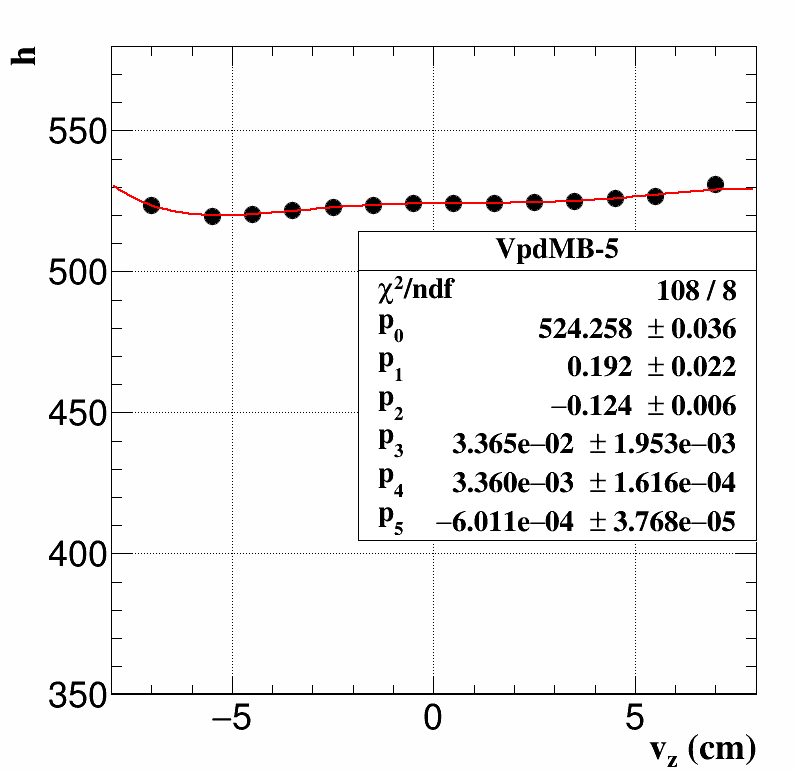
\includegraphics[width=0.75\textwidth]{figure/Run14_D0HFT/MB5_Vzcor2.png}
\caption{High end point as function of $V_{z}$ before correction.\label{fig:MB5_vz2}}
\end{minipage}
\hfill
\begin{minipage}[htbp]{0.52\linewidth}
\centering
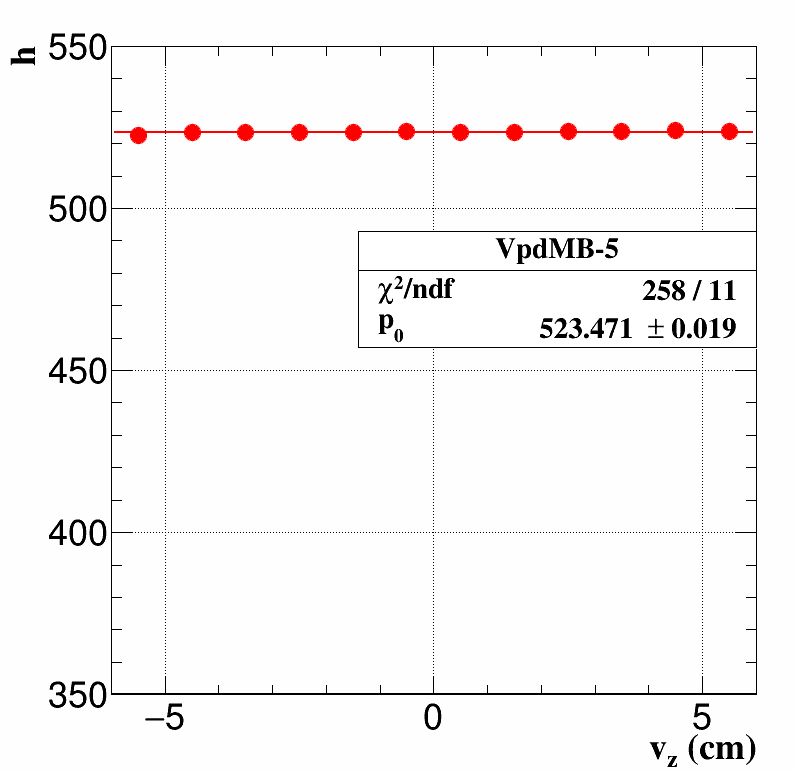
\includegraphics[width=0.75\textwidth]{figure/Run14_D0HFT/MB5_Vzcor3.png} 
\caption{High end point  as function of $V_{z}$ after correction.\label{fig:MB5_vz3}}
\end{minipage}
\end{figure}

As shown from Fig.~\ref{fig:MB5_vz} and Fig.~\ref{fig:MB30_vz}, the clear $V_{z}$ dependence need to avoid for VpdMB5 trigger. So, the centrality definition for VpdMB5 trigger was normalized to VpdMB30. After the ZdcX correction and $V_{z}$ correction, we directly take it as an additional correction factor for VpdMB5. These correction factor was show in Fig.~\ref{fig:MB5_vzscale}. After this additional correction, the distributions from VpdMB5 and VpdMB30 are same.

\begin{figure}[htbp]
\centering
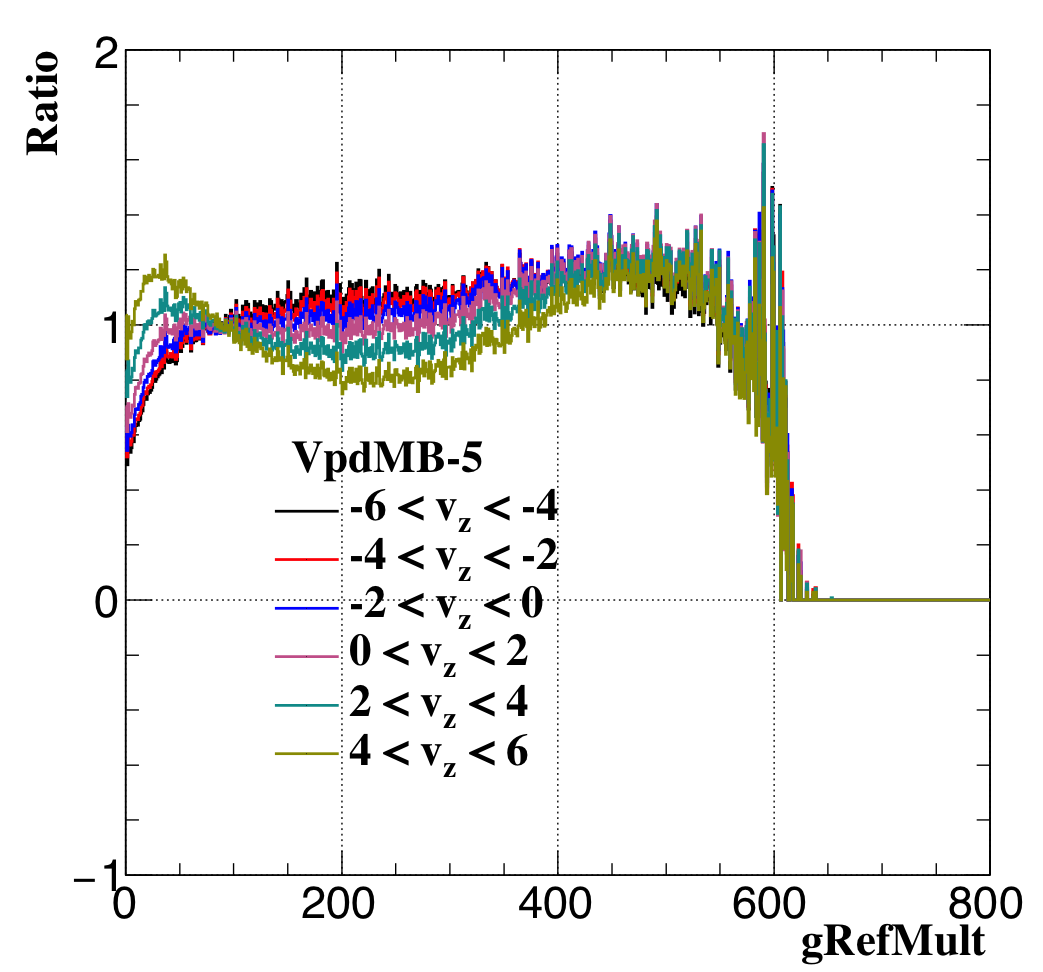
\includegraphics[keepaspectratio,width=0.5\textwidth]{figure/Run14_D0HFT/MB5_VzScale.png}
\caption{The double ratio of normalized gRefmult distribution from VpdMB5 over VpdMB30, this additional correction factor was try to normalized VpdMB5 to VpdMB30 trigger.}
 \label{fig:MB5_vzscale}
\end{figure}

The Vpd MinBias trigger has a trigger efficiency that are lower for periheral events. Fig.~\ref{fig:McData} shows the gRefmult after $V_{z}$ and ZdcX correction from data comparison with Glauber MC simulation. In the high end part the agreement was well, but in the low end part, due to this trigger ineffciency, there is clearly discrepancy between data and simulation. To do the measurement without centrality bias, a weight proportional to inverse trigger efficiency is applied. The weight as a function of corrected gRefMult is shown in Fig.~\ref{fig:vpdEffWeight}.

\begin{figure}[htbp]
\begin{minipage}[htbp]{0.52\linewidth}
\centering
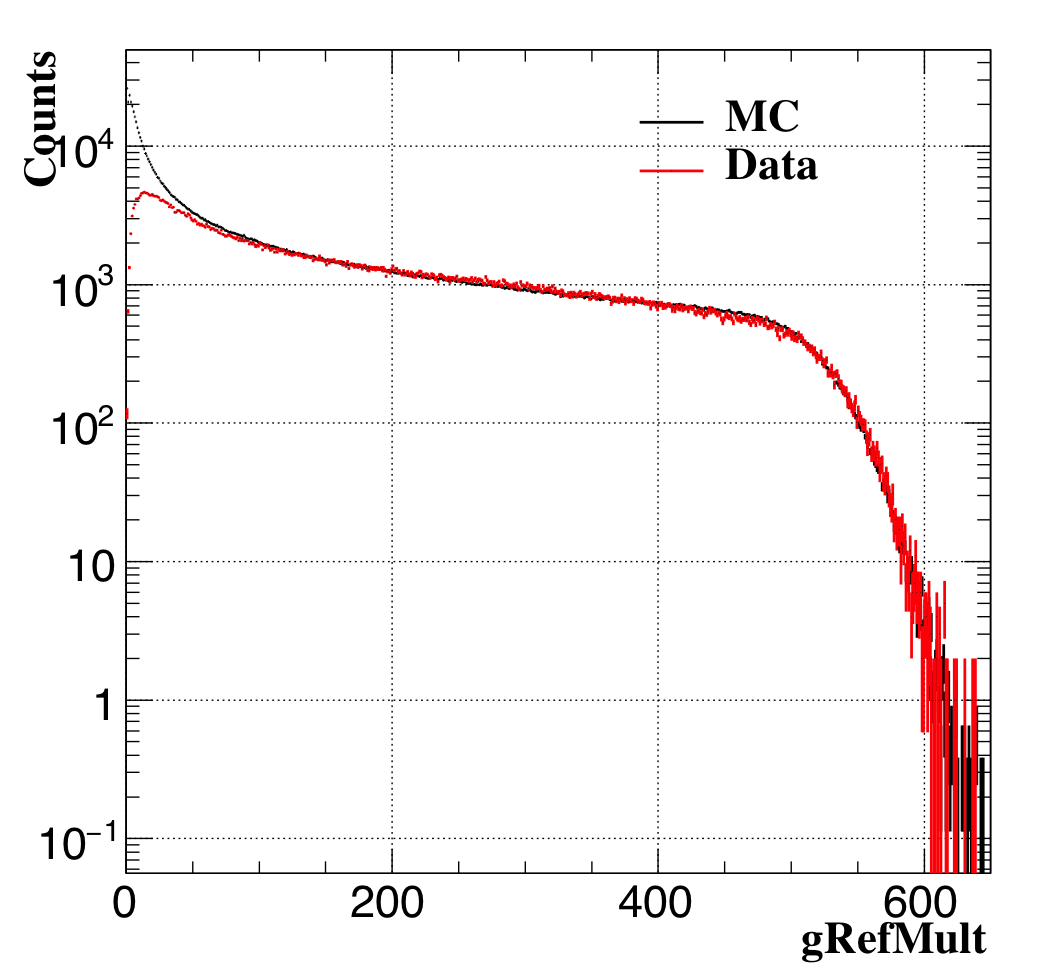
\includegraphics[width=0.75\textwidth]{figure/Run14_D0HFT/MB30_Mc_compare.png}
\caption{The comparison of corrected gRefMult between Data and Glauber MC. The red line is data and the black line is from Glauber MC.\label{fig:McData}}
\end{minipage}
\hfill
\begin{minipage}[htbp]{0.52\linewidth}
\centering
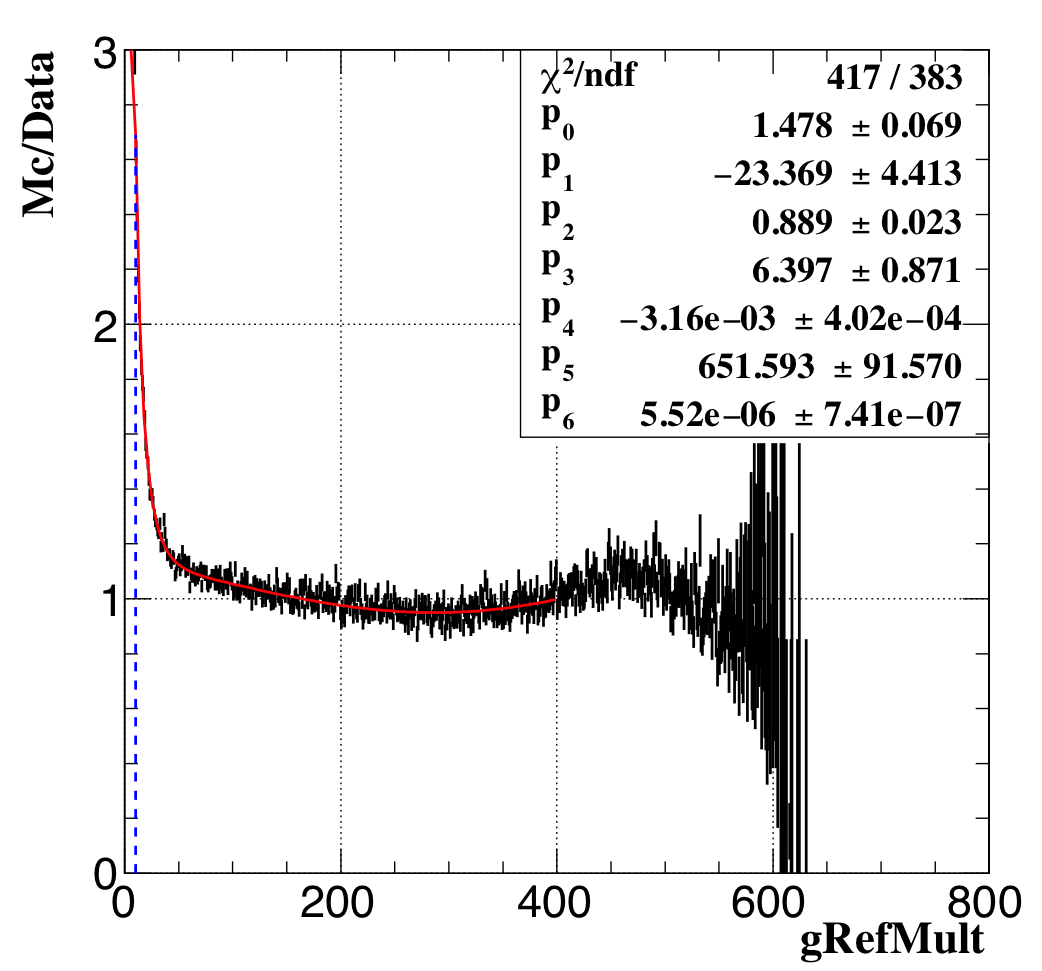
\includegraphics[width=0.75\textwidth]{figure/Run14_D0HFT/MB30_Mc_reweight.png} 
\caption{MC/data gRefmult distribution for Vpd MinBias trigger efficiency correction. The red line fit function is the correction reweight function.\label{fig:vpdEffWeight}}
\end{minipage}
\end{figure}

\begin{figure}[htbp]
\centering
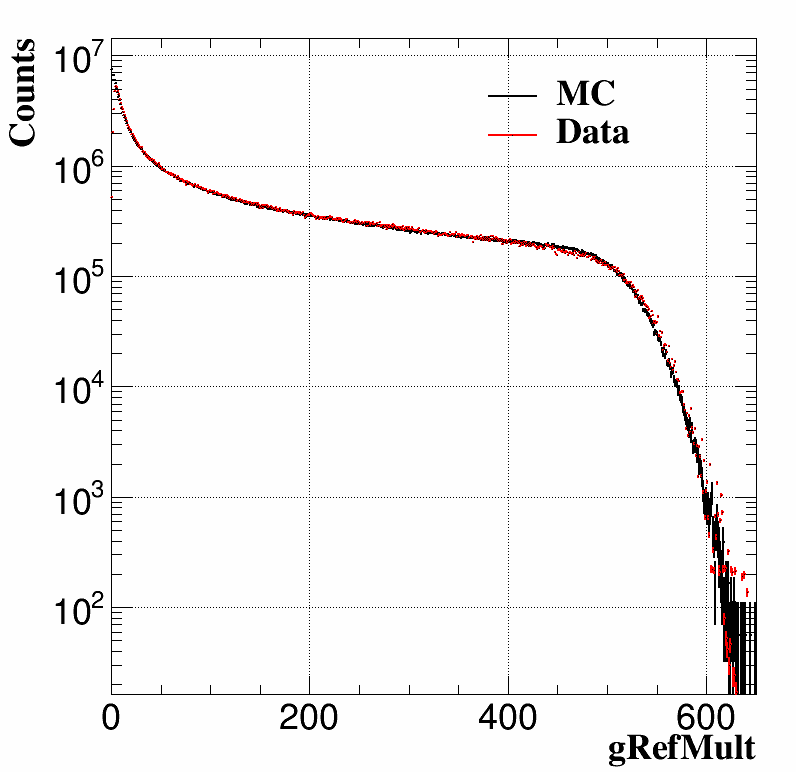
\includegraphics[keepaspectratio,width=0.5\textwidth]{figure/Run14_D0HFT/MB5_AfterALLMCData.png}
\caption{The comparison of corrected gRefMult (after all corrections and reweight) between Data and Glauber MC. The red line is data and the black line is from Glauber MC.\label{fig:MB5_afterAll}}
\end{figure}

After all these corrections including $V_{z}$, ZdcX, Vpd trigger inefficiency, and Vpd resolution for different centralities as discussed before. Final step, the data was compared to Glauber MC simulation as shown in Fig.~\ref{fig:MB5_afterAll}. And then the determined centrality classification can be found at Table ~\ref{centrality}.

\begin{table}[htp]
	\begin{center}
	\begin{tabular}{l|l|l|l}
  \toprule[1.6pt]
  \hline
  centrality & gRefMult & {$\langle$$N_{coll}$$\rangle$} & {$\langle$$N_{part}$$\rangle$} \\ \hline
  75-80$\%$ &	10-15	& 10.48 &	11.82 \\ \hline
	70-75$\%$ &	15-21	&	16.11 &	16.68 \\ \hline
	65-70$\%$ &	21-30	&	24.59 &	23.25 \\ \hline
	60-65$\%$ &	30-41	&	36.13 &	31.15 \\ \hline
	55-60$\%$ &	41-56	&	52.77 &	41.27 \\ \hline
	50-55$\%$ &	56-73	&	75.36 &	53.46 \\ \hline
  45-50$\%$ &	73-94	&	105.25 & 67.93 \\ \hline
  40-45$\%$ &	94-119 & 143.54 &	84.71 \\ \hline
  35-40$\%$ &	119-148	& 191.83 & 103.99 \\ \hline
	30-35$\%$ &	148-182	& 253.13 & 126.52 \\ \hline
	25-30$\%$ &	182-221	& 328.99 & 152.31 \\ \hline
	20-25$\%$ &	221-266	& 422.49 & 181.93 \\ \hline
	15-20$\%$ &	266-317	& 537.52 & 215.98 \\ \hline
	10-15$\%$ &	317-376	& 677.99 & 254.90 \\ \hline
	5-10 $\%$ &	376-443	& 852.75 & 299.95 \\ \hline
  0-5	 $\%$	& $>$443	& 1066.50	& 348.74 \\ \hline
  \hline
  \bottomrule[1.6pt]
	\end{tabular}
	\caption{Centrality defintion based on gRefMult}
	\label{centrality}
	\end{center}
\end{table}
